% !TEX root = ../../main.tex
% !TEX encoding = UTF-8 Unicode

%%%
\chapter{Physics Beyond the Standard Model}
\label{ch:limitations}

Although many predictions of the SM have been tested and verified, there are known issues that require extensions to the current theory. These proposed alterations are collectively known as beyond the standard model (BSM) theories. Many of these BSM theories in particular predict heavy resonances with couplings to the SM bosons. A ``heavy diboson resonance'' refers to the decay of such a resonance to a pair of SM bosons. In this chapter, several BSM theories which address shortcomings of the SM, and several benchmark models to test BSM physics are presented.

% Theory references for BSM
\section{Beyond the Standard Model}

In the SM, there are 19 free parameters which cannot be computed {\em a priori} and must be determined experimentally. The concept of ``naturalness'' dictates that these parameters should not require fine-tuning, and that dimensionless ratios of the parameters be of order unity. The mass of the Higgs has quadratically divergent loop corrections corresponding to the scale of any new physics, $\Lambda_{\text{cutoff}}$. 
$$m_H^2=m_{H,\text{bare}}^2+ \Delta m_H^2 = m_{H,\text{bare}}^2 + \alpha \Lambda_{\text{cutoff}}^2$$
The SM is expected to be accurate up to the Planck Scale, $\Lambda_{\text{Planck}}\sim 10^{19}\,\GeV$. However, in this case an incredible fine-tuning between the bare mass and the correction term is needed to recover the observed, $m_H^2\simeq 10^4\,\GeV$.  This fine-tuning violates the principle of naturalness and leads to the hierarchy problem: why is the weak scale, $\Lambda_{\text{EW}}$, so much lower than the Planck scale, $\Lambda_{\text{Planck}}$.

In an attempt to address the fine-tuning problem, composite Higgs models~\cite{comp_higgs_1,comp_higgs_2} propose a new strongly interacting sector with a larger symmetry group, and explain electroweak symmetry breaking without a fundamental scalar. By a careful choice of the new expanded symmetry group, spontaneous symmetry breaking in the new strongly interacting sector, at a scale $\Lambda_{\text{comp}}\ll \Lambda_{\text{Planck}}$, can produce a composite Goldstone boson transforming as the SM Higgs doublet, and an unbroken symmetry corresponding to the electroweak $SU(2)\times U(1)$ symmetry group. The larger global symmetry is also explicitly broken, such as with Yukawa and gauge coupling terms, so that the Goldstone boson corresponding to the composite Higgs is no longer exactly massless.
%\footnote{The massive Goldstone boson that arises due to both explicit and spontaneous breaking of a continuous global symmetry is called a pseudo-Goldstone boson. }
The approximate symmetry of the new sector keeps the Higgs mass low, addressing the issue of naturalness.  Among the predictions of these models is resonances of composite scalars and new heavy gauge bosons near the \TeV\,scale.  

Another attempt at addressing the hierarchy problem is by postulating warped extra dimensions~\cite{warped_xtra_dim_1,warped_xtra_dim_2,warped_xtra_dim_3}, referred to as Randall-Sundrum (RS) models. In these theories, the universe is embedded in a five dimensional space (bulk) with constant negative scalar curvature (anti-de Sitter).
%\footnote{ Anti-de Sitter space has a constant negative scalar curvature, and is sometimes referred to as ``hyperbolic'' space.}
The SM particles are localized on a ($3+1$)-dimensional subspace (3-brane), called the weak or \TeV\, brane, while there is a separate 3-brane where gravity is relatively strong, called the Planck brane. Only gravity is able to propagate in the bulk through the extra dimension.
%\footnote{In an attempt to unite Einstein's gravitational field equations with electromagnetism, the KK model introduced a periodic fifth dimension, $\phi\sim \phi+2\pi R$, as a factorizable extension to Minkowski space: the bulk is a five dimensional cylinder of radius $R$ which can be compactified as $R\ra0$.}
The RS five dimensional metric is non-factorizable: the flat 4D Minkowski metric, $\eta_{\mu\nu}=\textrm{diag}(-1,1,1,1)$, has an additional ``warping'' factor that explicitly depends on the extra dimension, $\phi$, as shown in~\Eqn{\ref{eq:rs_metric}} for the space-time interval, $ds^2$. Here, $x^{\mu}$ are the familiar four-dimensional space-time coordinates.
\begin{equation}
ds^2=e^{-2kr_c|\phi|}\eta_{\mu\nu}dx^{\mu}dx^{\nu}+ r_c^2d\phi^2
\label{eq:rs_metric}
\end{equation}
The curvature scale, $k$, is assumed to be of order the Planck scale, and the compactification radius, $r_c$, determines the size of the extra dimension.
%\footnote{A second model in the limit $r_c\ra\infty$ also resolves the hierarchy problem. In this case, one of the branes is taken to infinity, effectively leaving only one brane.} 
By placing the Planck brane at $\phi=0$ and the weak brane at $\phi=\pi$, physical mass parameters on the weak brane accumulate a warping factor with respect to their higher dimensional values, $m=e^{-kr_c\pi}m_0$, while the Planck scale on a brane depends only weakly on the fifth dimension. Provided $kr_c\simeq 12$, the observed hierarchy on the weak brane emerges geometrically from the warped extra dimension, as depicted in~\Fig{\ref{fig:rs_branes}}. RS models predict Kaluza-Klein (KK) excitations~\cite{kaluza_klein_mode},
%\footnote{In the Kaluza Klein model, a massless scalar $\phi(x^{\mu},x^5)$ has quantized motion in the periodic dimension: $p^5 = \frac{n}{R}$. A Fourier expansion of the field in the fifth dimension yields, $\phi(x^{\mu},x^5)=\sum_n\phi^n(x^{\mu})e^{inx^5/R}$. An equation of motion for $\phi$ in ($3+1$) dimensions can be given:
%$$\left(\partial_{\mu}\partial^{\mu} + \partial_5\partial^5\right)\phi = 0\quad\quad \Rightarrow \partial_{\mu}\partial^{\mu}\phi^n(x^{\mu})=\frac{n^2}{R^2}\phi^n(x^{\mu})$$
%This describes an infinite tower of fields $\phi^n(x^{\mu})$ with masses $m^2=\frac{n^2}{R^2}$. For higher spin fields, the procedure is more complicated but a similar reduction produces a tower of massive KK excitations~\cite{kaluza_klein_mode}.}
from the massless graviton propagating in the extra dimension, coupling to SM gauge bosons; notably, the lowest modes are expected near the \TeV\, scale where their masses and couplings are determined.

\begin{figure}[tbp]
\begin{center}
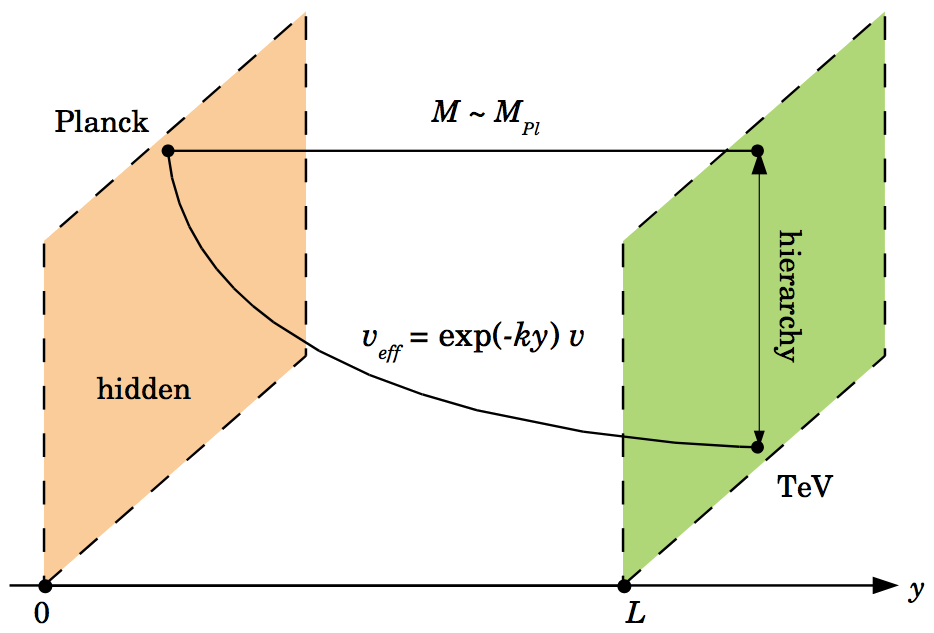
\includegraphics[width=0.7\textwidth]{figures/StandardModel/rs_branes}
\end{center}
\caption[Schematic of warped extra dimensions]{In the RS model, a Planck brane and weak brane are separated by a warped extra dimension. The Planck scale on a brane only weakly depends on the extra dimension, while the mass scales receive a warping factor~\cite{rs_pic}.}
\label{fig:rs_branes}
\end{figure} 

Spontaneous symmetry breaking in the SM, with a single complex scalar transforming as a weak isospin doublet, is a minimal solution to provide mass to gauge bosons in the electroweak sector, in a gauge invariant way. As a result, the minimal Higgs sector of the SM purports to simultaneously address two disparate problems: the weak gauge bosons acquire mass by ``eating'' degrees of freedom from the complex scalar, and all fermions acquire mass by Yukawa couplings placed by hand.  Theories with an extended Higgs sector~\cite{extended_higgs_1, extended_higgs_2} preserve all of the SM gauge symmetries while splitting the functions of the SM doublet between multiple doublets, with some proposing even more exotic extensions with scalars transforming as weak isospin singlets or triplets. The simplest extensions, called $N$ Higgs doublet models (NHDM), propose $N$ complex scalar fields transforming as weak isospin doublets with weak hypercharge $Y=1$. For example, with $N=2$, the two complex scalar doublets describe eight real scalars: three generate mass for the weak bosons, three correspond to neutral scalars,
%\footnote{One must correspond to the 125\,\GeV\, SM Higgs. Depending on the mixing of the neutral scalars and required symmetries, the 2HDM can either conserve or violate CP.}
and two correspond to charged Higgs. In addition to spreading the Yukawa couplings among additional doublets, extended Higgs sector theories can offer mechanisms for CP violation; the singlet extension can explain dark matter;
%\footnote{If the singlet extension does not mix with the SM Higgs, it would have no interactions with the gauge bosons and fermions. It could be a window into a ``dark sector'', only interacting with the SM sector via a term like $\lambda \phi^{\dagger}\phi|S|^2$, where $S$ is the new singlet scalar.}
and a triplet extension can explain neutrino masses without introducing a right-handed neutrino.
%\footnote{The process is known as the Type II Seesaw Mechanism.}
New resonances in an extended Higgs sector offer a rich phenomenology through couplings to the massive weak bosons.   


While the electromagnetic and weak interactions in the SM unify in the electroweak sector,
%\footnote{However, they are ``unified'' in a slightly unsatisfactory way as two separate gauge couplings are required.} 
the strong sector and electroweak sector commute. The innate intuition,
%\footnote{One might even say GUT feeling.}
or perhaps desire, that there should be fundamental symmetries is at slight conflict with the {\em ad hoc} fashion in which the SM gauge group glues together the otherwise separate strong and electroweak sectors. Grand Unified Theories~\cite{gut_1, gut_2, gut_3, gut_4} (GUT) embed the SM gauge group in a single larger group, whereby the strong and electroweak interactions unify at a large scale, $\Lambda_{\text{GUT}}$, manifesting themselves as separate interactions at lower energies. The running of the three gauge couplings shows a curious near convergence, motivating $\Lambda_{\text{GUT}}\simeq10^{16}\,\GeV$.
%\footnote{The convergence can be made exact with the addition of Supersymmetry~\cite{Zee}.}
In addition to the overt goal of unification, GUTs generally offer a mechanism for electric charge quantization, and specifically an explanation for why protons and electrons have exactly opposite charges. Among the challenges of GUTs, the prediction of magnetic monopoles and of proton decay
%\footnote{In the higher gauge group, leptons and quarks generally mix through the exchange of new heavy vector bosons, violating baryon number conservation.} 
is strongly constrained by experiment. The simplest such theory involves the group $SU(5)$, although there is no single accepted formulation; notably, $SO(10)$ requires no extra fermions, and features each generation transforming in one irreducible multiplet.
%\footnote{The fermions transform as a spinor in the $\mathbf{16}$ representation, exactly fitting the 16 fermions of each generation: $u^{r,g,b}_L, d^{r,g,b}_L, (u^c_L)^{r,g,b}, (d^c_L)^{r,g,b}, e_L, e^c_L, \nu_L, \nu_L^c$~\cite{Zee}. The right-handed neutrino, $\nu_L^c$, is a small extension of the SM explaining neutrino masses, and a singlet under the SM gauge group.}
In GUTs, a large number of new gauge bosons are predicted, corresponding to the generators of the larger symmetry group. Since the larger symmetry is not realized at the electroweak scale, a series of symmetry breaking scales reduces the larger symmetry to the observed SM gauge group, while the gauge bosons of the broken symmetries acquire mass near the symmetry breaking scales. 


% Benchmark theory references
\section{Benchmark Models of New Physics}

Exploiting the predicted coupling of new resonances to weak SM gauge bosons in several well-motivated BSM theories, this thesis searches for a resonant peak in $WV$ ($V=W,Z$) production. In particular, the semi-leptonic final state ($\ell\nu qq$) of the diboson resonance is chosen as a balance between a higher branching ratio and a cleaner signal: the leptonically decaying $W\ra \ell\nu$ ($\ell = e, \mu$) is cleanly reconstructed by the detector but has a small branching ratio of $21.3\,\%$, while the hadronically decaying $V\ra q\overline{q}'/q\bar{q}$ ($q,q'=u,d,c,s,b$) is more difficult to reconstruct but has a large branching ratio of $69.9\,\%\, (67.4\,\%)$ for the $Z\, (W)$ channel~\cite{pdg_2017}.
%\footnote{In the LHC, protons are collided which are composed principally of quarks ($uud$) and not antiquarks, although at higher energies, quark anti-quark pairs begin to populate the proton. As a result, quark scattering and diffraction creates a very noisy background for the hadronically decaying $V$, while leptons are comparatively rarely produced from $q\bar{q}'$ interactions due to the low population of anti-quarks.}
For heavy new resonances, the opening angle between the two quarks from the hadronically decaying $V$ boson is small.  This thesis explores the so-called ``boosted'' regime where the opening angle between the quarks is small enough that they are reconstructed as one object, denoted $J$ (jet). In the rest of this thesis, the search for a diboson resonance in the boosted semi-leptonic final state channel will be abbreviated as $WV\ra \ell\nu J$.
%\footnote{The measurement of hadronic and leptonic jets in the detector is discussed in~\Sect{\ref{ch:atlas:particle_showers}}, while the reconstruction of objects from detector data is discussed in~\Ch{\ref{ch:objreco}}. The boosted regime is described in more detail in~\Ch{\ref{ch:event_selection}}.} 
Several benchmark BSM models, which include spin-0, spin-1, or spin-2 bosons decaying to $WW$ or $WZ$, are used to interpret the results of the search and quantify the sensitivity. The models are listed in~\Tab{\ref{tab:bench_models}}, with Feynman diagrams depicting the principal production channels. 

\begin{table}[tbp]
\begin{center}
\begin{tabular}{ccc}
\hline\hline
Model & Production & Diagram \\ \hline
\vbox{\hbox{\strut }\hbox{\strut \textbf{Scalar Heavy Higgs}}\hbox{\strut Spin-0}}  & $ggF$ & \feynmandiagram[baseline=(c.base), horizontal=c to d] {
i1 [particle=\(g\)] -- [gluon] a, 
i2 [particle=\(g\)] -- [gluon] b,
i1 -- [draw=none] i2,
a -- [fermion, edge label={\( t, b\)}] b -- [fermion] c -- [fermion] a,
c -- [scalar, edge label={\(H\)}] d,
f1 [particle=\(W^{\pm}\)] -- [boson] d -- [boson] f2 [particle={\(W^{\mp}\)}],
}; \\ \cline{2-3}
& VBF & \feynmandiagram[layered layout, baseline=(b.base), vertical=t1 to n2, sibling distance=1cm] {
   g1 [particle=\(q\)]
     -- [fermion] a
     -- [fermion] t1 [particle=\(q'\)],
  { [same layer]
    c -- [boson, edge label=\(V\)] b
      -- [boson, edge label=\(V\)] a},
   b  -- [scalar, edge label={\(H\)}] n2,
   n2 -- [boson] n1 [particle=\(W^{\pm}\)],
   n2 -- [boson] n3 [particle={\(W^{\mp}\)}],
   g2 [particle=\(q\)]
      -- [fermion] c
      -- [fermion] t2 [particle=\(q'\)],
 }; \\ \hline
\vbox{\hbox{\strut }\hbox{\strut \textbf{Heavy Vector Triplet}}\hbox{\strut \textbf{(HVT)}}\hbox{\strut Spin-1}} &$q\bar{q}$ & \feynmandiagram [baseline=(a.base), horizontal=a to b] {
i1 [particle=\(q\)] -- [fermion] a -- [fermion] i2 [particle=\(\bar{q}\)],
a -- [boson, edge label={\(W', Z'\)}] b,
f1 [particle=\(W^{\pm}\)] -- [boson] b -- [boson] f2 [particle={\(Z, W^{\mp}\)}],
};\\ \cline{2-3}
\vbox{\hbox{\strut Model-A: $g_V = 1$}\hbox{\strut }\hbox{\strut Model-B: $g_V = 3$}\hbox{\strut }}&VBF & \feynmandiagram[layered layout, baseline=(b.base), vertical=t1 to n2, sibling distance=1cm] {
   g1 [particle=\(q\)]
     -- [fermion] a
     -- [fermion] t1 [particle=\(q'\)],
  { [same layer]
    c -- [boson, edge label=\(V\)] b
      -- [boson, edge label=\(V\)] a},
   b  -- [boson, edge label={\(W', Z\)}] n2,
   n2 -- [boson] n1 [particle=\(W^{\pm}\)],
   n2 -- [boson] n3 [particle={\(Z, W^{\mp}\)}],
   g2 [particle=\(q\)]
      -- [fermion] c
      -- [fermion] t2 [particle=\(q'\)],
 };\\ \hline
\vbox{\hbox{\strut }\hbox{\strut \textbf{Bulk Randall-Sundrum}}\hbox{\strut \textbf{(RS) Graviton}}\hbox{\strut Spin-2}\hbox{\strut }\hbox{\strut $\frac{k}{\overline{M}_{\textrm{Pl}}}=1.0, 0.5$}} & $ggF$ & \feynmandiagram [baseline=(a.base),horizontal=a to b] {
i1 [particle=\(g\)] -- [gluon] a -- [gluon] i2 [particle=\(g\)],
a -- [boson, edge label={\(G^*\)}] b,
f1 [particle=\(W^{\pm}\)] -- [boson] b -- [boson] f2 [particle={\(W^{\mp}\)}],
}; \\
\hline\hline 
\end{tabular}
\caption[Benchmark signal models and leading order Feynman diagrams]{The benchmark signal models used in the analysis are shown. The spin-0 interpretation is a neutral Higgs-like scalar decaying to two $W$ bosons, produced either by gluon-gluon fusion ($ggF$) or vector boson fusion (VBF). Two heavy vector triplet (HVT) models are considered, with new spin-1 bosons, $W'$ and $Z'$, produced either by quark-quark fusion ($q\bar{q}$) or VBF, and decaying via $W'\ra WZ$ or $Z'\ra WW$.  In Model-A, $g_V=1$ and couplings to fermions are comparable to those of gauge bosons. In Model-B, $g_V=3$ and fermionic couplings are suppressed. The spin-2 bulk Randall-Sundrum (RS) Graviton, produced via ggF and decaying to two $W$ bosons, is examined for values $k/\overline{M}_{\textrm{Pl}}=1.0, 0.5$. }
\label{tab:bench_models}
\end{center}
\end{table}

A neutral, scalar heavy Higgs~\cite{heavy_higgs_1, heavy_higgs_2} is considered to model a spin-0 resonance decaying to $WW$. Such scalar resonances are predicted by several theories of an extended Higgs sector. The scalar is modeled as a Breit-Wigner resonance using a narrow width approximation (NWA)~\cite{nwa_info}.
%\footnote{The NWA is when the width is much smaller than the pole mass, $\Gamma\ll M$, and is useful for factorizing the production from the subsequent decay by assuming the total cross section is dominated by on-shell resonances~\cite{nwa_info}.}
The width of the resonance is taken to be less than the detector resolution and set to $4\,\MeV$. The NWA neglects any interference between the resonance and SM diboson production. Although the heavy Higgs does not couple to gluons directly, gluon-gluon fusion (ggF) through a quark loop (see~\Tab{\ref{tab:bench_models}}) is the dominant production mechanism at the LHC. Vector boson fusion (VBF) production is also considered: the final state is distinguished from that of ggF production by the hadronization of the two initial quarks radiating vector bosons, reconstructed as additional forward jets. These two production mechanisms are simulated separately~\cite{heavy_higgs_ggF, heavy_higgs_VBF}.

Charged or neutral spin-1 resonances decaying to $WW$ or $WZ$ are predicted by many BSM theories with extended gauge symmetries or a new strongly interacting sector, including GUTs, theories of extra dimensions, and composite Higgs models. To extend the applicability of the results, a phenomenological Lagrangian is considered that involves only those parameters which determine the mass and relevant couplings of the resonance. A heavy vector triplet (HVT) model~\cite{hvt_theory_1, hvt_theory_2} with a simplified Lagrangian is considered with three new gauge bosons, $W'^{\pm}$ and $Z'$, transforming in the adjoint representation of $SU(2)_L$ as a weak-isospin triplet with hypercharge $Y=0$. 
The relative strength of the new vector boson interaction is described by a parameter $g_V$, and dimensionless factors $c_F$ and $c_H$ describe the deviation from typical values of the new boson coupling to fermions and SM gauge bosons, respectively. The coupling of the new triplet to the SM Higgs and weak gauge bosons is described by the parameter combination $g_Vc_H$, while the coupling of the new triplet to SM fermions is parameterized by the combination $g^2c_F/g_V$, where $g$ is the SM $SU(2)_L$ coupling. 
%Both $c_F$ and $c_H$ are taken to be $\simeq 1$. 
In general, the parameter $c_F$ can be different for leptons, light quarks, and third generation quarks, but is taken to be universal in this simplified model, with $c_F\sim 1$~\cite{hvt_theory_1}. Couplings involving two or more new vector bosons are neglected.
%\footnote{Other parameters like $c_{VVV},  c_{VVHH}$, and $c_{VVW}$ describe interactions which have a negligible contribution to the production and decay process involved in this analysis.}
Two models, corresponding to a weak and a strong interaction of the new vector bosons, are considered. To characterize a theory with an extended gauge group~\cite{hvt_model_a, hvt_model_a2}, model-A has $c_H\simeq g^2/g_V$ and fixes $g_V=1$: fermions and gauge bosons have similar couplings to the new triplet ($g_Vc_H\simeq g^2c_F/g_V$). Conversely, model-B has $c_H\simeq 1$ and fixes $g_V=3$, describing a strongly interacting composite Higgs theory~\cite{hvt_model_b_1,hvt_model_b_2, hvt_model_b_3}. Consequently, the fermionic coupling to the new vector bosons in model-B is suppressed ($g^2c_F/g_V \ll g_Vc_H$). The HVT is primarily produced by quark-quark fusion ($q\bar{q}\ra Z'$ or $q\bar{q}'\ra W'$). VBF production is generally suppressed;
%\footnote{With respect to quark-quark fusion, VBF requires two extra weak interactions, and thus is suppressed by $\frac{1}{\alpha_{EW}^2}$.}
however, if the coupling of the HVT to fermions is anomalously small, $c_F\simeq 0$, VBF production is dominant. Therefore, both production mechanisms are considered for both models. 

A neutral, spin-2 resonance decaying to $WW$ is predicted by Randall-Sundrum (RS) theories of warped extra dimensions. In this search, a bulk RS model~\cite{rs_graviton} extension of the original RS model is used, where the SM fields are allowed to propagate in the higher dimensional bulk, except for the Higgs field which remains constrained to the \TeV\, brane. In this formulation, since the SM fields no longer reside on the \TeV\, brane, their localization in the bulk can reproduce the observed flavor hierarchy. Particles residing closer to the Planck brane have lighter masses on the \TeV\, brane due to the warping factor. The RS graviton is realized on the \TeV\, brane as the first KK excitation~\cite{kaluza_klein_mode}.
%\footnote{The $n^{\textrm{th}}$ KK excitation mode produces one spin-2 resonance, $(n-1)$ spin-1 resonances which decouple, and $\frac{n(n-1)}{2}$ spin-0 resonances, all with the same mass~\cite{kaluza_klein_mode}.}
In the bulk RS model, since the light fermions are localized far from the \TeV\, brane, the graviton KK excitation on the \TeV\, brane is minimally coupled to them. As a result, ggF is the dominant production mechanism considered. Longitudinal $W_L/Z_L$ decay modes are enhanced by the strong coupling of the KK excitation to the Higgs field.
%\footnote{For large energies, the longitudinally polarized $W_L/Z_L$ bosons correspond to the Goldstone bosons of the doublet Higgs field~\cite{rs_graviton}.}
The width of the first KK excitation is proportional to $(k/\overline{M}_{\textrm{Pl}})^2$, where $k$ is the curvature scale and $\overline{M}_{\textrm{Pl}}=M_{\textrm{Pl}}/\sqrt{8\pi}$ is the reduced Planck mass~\cite{grav_width}. 
%To solve the hierarchy problem, $kr_c\simeq12$; thus smaller values of $k/\overline{M}_{\textrm{Pl}}$ imply large $r_c$. 
Large values of $k/\overline{M}_{\textrm{Pl}}$ cause the theory to be non-perturbative (ratio must be approximately $<3.0$~\cite{rs_graviton}). Even in the perturbative regime, larger values of the ratio inflate the width of the resonance (for $k/\overline{M}_{\textrm{Pl}}\sim2$, the width is approximately 20\,\% the mass of the resonance). In this thesis, values of  $k/\overline{M}_{\textrm{Pl}}$ equal to $1.0$ and $0.5$ are considered.






